%!TEX root = ./RfCPN.tex


\addtocontents{toc}{\protect\cleardoublepage}
%%%%%%%%%%%%%%%%%%%%%%%%%%%%%%%%%%%%%%%%%%%%%%%%%%%%%%%%%
%% Part Requirement Definition %%%%%%%%%%%%%%%%%%%%%%%%%%
%%%%%%%%%%%%%%%%%%%%%%%%%%%%%%%%%%%%%%%%%%%%%%%%%%%%%%%%%
\addtocontents{toc}{\protect\begin{tocBox}{\tmppartnum}}%
\tPart[lof]{機械の稼働における\index{きのうせっけい@機能設計}機能設計\TBW}{%
\paragraph*{\tpartgoal}
新たな横型マシニングセンタの稼働に向けて、\index{システムせっけい@システム設計}システム設計(\index{きのうせっけい@機能設計}機能設計)を行う。

\tcbline*
\paragraph*{\tpartmethod}
特定された\index{ようけん@要件}要件を基に、\index{きのうせっけい@機能設計}機能設計を行う。

\tcbline*
\paragraph*{\tpartbackground}
先にも述べたとおり、\index{システムかいはつプロセスのけいかく@システム開発プロセスの計画}システム開発プロセスの計画は白紙状態であるが、とにかく稼働をさせ生産のできる状態にすることが喫緊の課題である。

 その一環として、前段階の特定された\index{ようけん@要件}要件を用いて、機械の稼働における\index{きのうせっけい@機能設計}機能設計を速やかに行う必要がある。
}{%
\paragraph*{\tpartconclusion}
(to be written...)
\tcbline*
\paragraph*{\tpartnextstep}
(to be written...)
}

%%%%%%%%%%%%%%%%%%%%%%%%%%%%%%%%%%%%%%%%%%%%%%%%%%%%%%%%%
%% chapters %%%%%%%%%%%%%%%%%%%%%%%%%%%%%%%%%%%%%%%%%%%%%%
%%%%%%%%%%%%%%%%%%%%%%%%%%%%%%%%%%%%%%%%%%%%%%%%%%%%%%%%%%
\modHeadchapter[lof]{システムの全体像\TBW}
% システムが達成すべき全体的な目標と要件を説明



\modHeadsection{システムの目的\TBW}
(to be written...)



\modHeadsection{システムの主要な機能\TBW}
(to be written...)


%%%%%%%%%%%%%%%%%%%%%%%%%%%%%%%%%%%%%%%%%%%%%%%%%%%%%%%%%%
%% figure %%%%%%%%%%%%%%%%%%%%%%%%%%%%%%%%%%%%%%%%%%%%%%%%
%%%%%%%%%%%%%%%%%%%%%%%%%%%%%%%%%%%%%%%%%%%%%%%%%%%%%%%%%%
\begin{figure}[p]%
\begin{Figlandscape}
\begin{adjustbox}{%
  addcode={\begin{minipage}{\textheight}\centering}{%
    \captionof{figure}{加工全体のフロー(概要)\label{fig:flowchart}}%
    \end{minipage}%
  },
  rotate=90,
  center,
%  max width=\textheight,
%  max height=\linewidth,
  keepaspectratio}
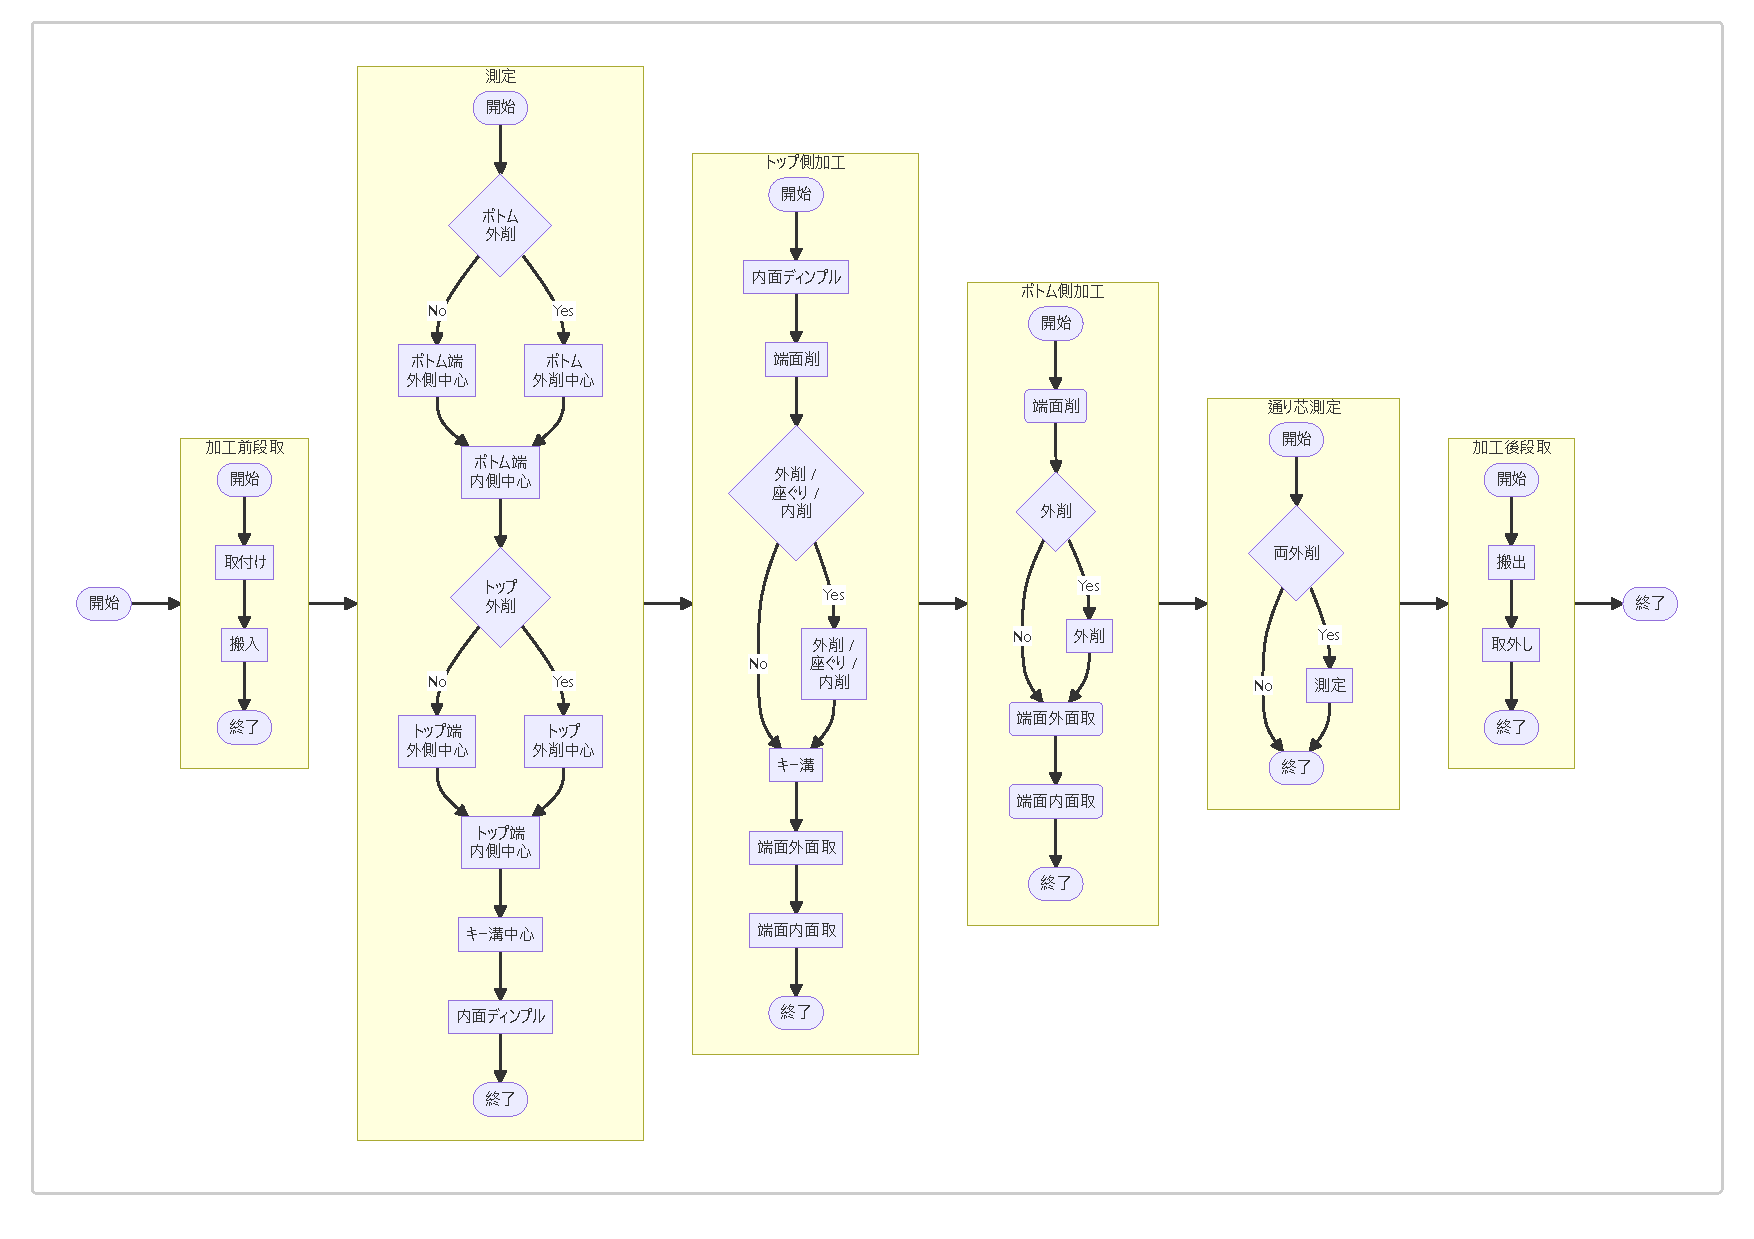
\includegraphics[height=\linewidth-10pt, trim=20 30 20 20, clip]{RfCPN_p03_pictures/Milling_flow_chart.pdf}%
\end{adjustbox}
\end{Figlandscape}%
\end{figure}%
%%%%%%%%%%%%%%%%%%%%%%%%%%%%%%%%%%%%%%%%%%%%%%%%%%%%%%%%%%
%%%%%%%%%%%%%%%%%%%%%%%%%%%%%%%%%%%%%%%%%%%%%%%%%%%%%%%%%%
%%%%%%%%%%%%%%%%%%%%%%%%%%%%%%%%%%%%%%%%%%%%%%%%%%%%%%%%%%




\modHeadchapter{主要な機能\TBW}
% システムの主要な機能を詳細に説明



\modHeadsection{機能1の詳細\TBW}
(to be written...)



\modHeadsection{機能2の詳細\TBW}
(to be written...)




\modHeadchapter{機能間の相互作用\TBW}
% 機能がどのように相互作用するかを説明



\modHeadsection{機能1と機能2の相互作用\TBW}
(to be written...)



\modHeadchapter{ユーザーとの対話\TBW}
% ユーザーがシステムとどのように対話するかを説明



\modHeadsection{ユーザーインターフェースの設計\TBW}
(to be written...)



\modHeadsection{ユーザーの操作フロー\TBW}
(to be written...)

%%%%%%%%%%%%%%%%%%%%%%%%%%%%%%%%%%%%%%%%%%%%%%%%%%%%%%%%%
%% Appendices %%%%%%%%%%%%%%%%%%%%%%%%%%%%%%%%%%%%%%%%%%%
%%%%%%%%%%%%%%%%%%%%%%%%%%%%%%%%%%%%%%%%%%%%%%%%%%%%%%%%%
\begin{appendices}
%\Appendixpart
\end{appendices}

\addtocontents{toc}{\protect\end{tocBox}}
